\documentclass{standalone}
\usepackage[T1]{fontenc}
\usepackage[latin2]{inputenc}
\usepackage[english]{babel}
\usepackage{tikz}
\usepackage{times}

% Packages needed to draw 
\usetikzlibrary{calc,through,backgrounds,positioning,fit}
\usetikzlibrary{shapes,arrows,shadows}
 
\begin{document}
 
% Defining different types of nodes %%%%%%%%%%%%%%%%%%%%%%%%%%%%%%%%%
\tikzstyle{place}=[shape=circle, draw, minimum height=10mm]
\tikzstyle{trig}=[shape=circle, draw, dashed, minimum height=10mm]
\tikzstyle{trans}=[shape=rectangle, draw, minimum height=6mm, minimum width=12mm]
 
\centering

%OPTIONS of tikzpicture:
% scale option scales the whole picture 


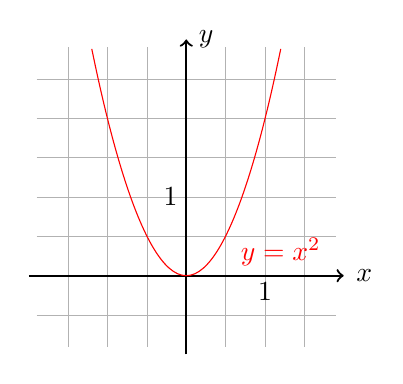
\begin{tikzpicture}[scale=1,inner sep=0.4mm]

\draw[step=5mm,draw=black!30!white,very thin] (-1.9,-0.9) grid (1.9,2.9);


% Draw coordinate system %%%%%%%%%%%%%%%%%%%%%%%%%%%%%%%%%%%%%%%%%%%%%
\draw[thick] [->] (-2,0) -- (2,0) node [right=3pt] {$x$};
\draw[thick] [->] (0,-1) -- (0,3) node [right=3pt] {$y$};
 			
     			

% Draw chart %%%%%%%%%%%%%%%%%%%%%%%%%%%%%%%%%%%%%%%%%%%%%%%%%%%%%%%%
\draw [red] (0,0) parabola (1.2, 2.88);
\draw [red] (0,0) parabola (-1.2,2.88);

% Set a label for chart %%%%%%%%%%%%%%%%%%%%%%%%%%%%%%%%%%%%%%%%%%%%%
\node [red] at (1.2,0.3) {$y=x^{2}$};
\node at (1,-0.2) {$1$};
\node at (-0.2,1) {$1$};



\end{tikzpicture}
 
\end{document}